% \Image{Capa do livro (; )}{PNLD2022-020-01.png}

% \Image{Ilustração do livro (; )}{PNLD2022-020-04.png}
% \Image{Ilustração do livro (; )}{PNLD2022-020-05.png}
% \Image{Ilustração do livro (; )}{PNLD2022-020-06.png}


\documentclass[11pt]{extarticle}
\usepackage{manualdoprofessor}
\usepackage{fichatecnica}
\usepackage{lipsum,media9}
\usepackage[justification=raggedright]{caption}
\usepackage[one]{bncc}
\usepackage[ubu]{../edlab}
\usepackage{marginnote}
\usepackage{pdfpages}
\usepackage[printwatermark]{xwatermark}
%\newwatermark[pagex=2]{
\includegraphics[scale=3.3]{watermarks/test-a.png}}	% página específica
%\newwatermark[oddpages]{
\includegraphics{watermarks/test-a.png}}			% páginas ímpars
%\newwatermark[evenpages]{
\includegraphics{watermarks/test-a.png}}			% págimas pares
\newwatermark[allpages]{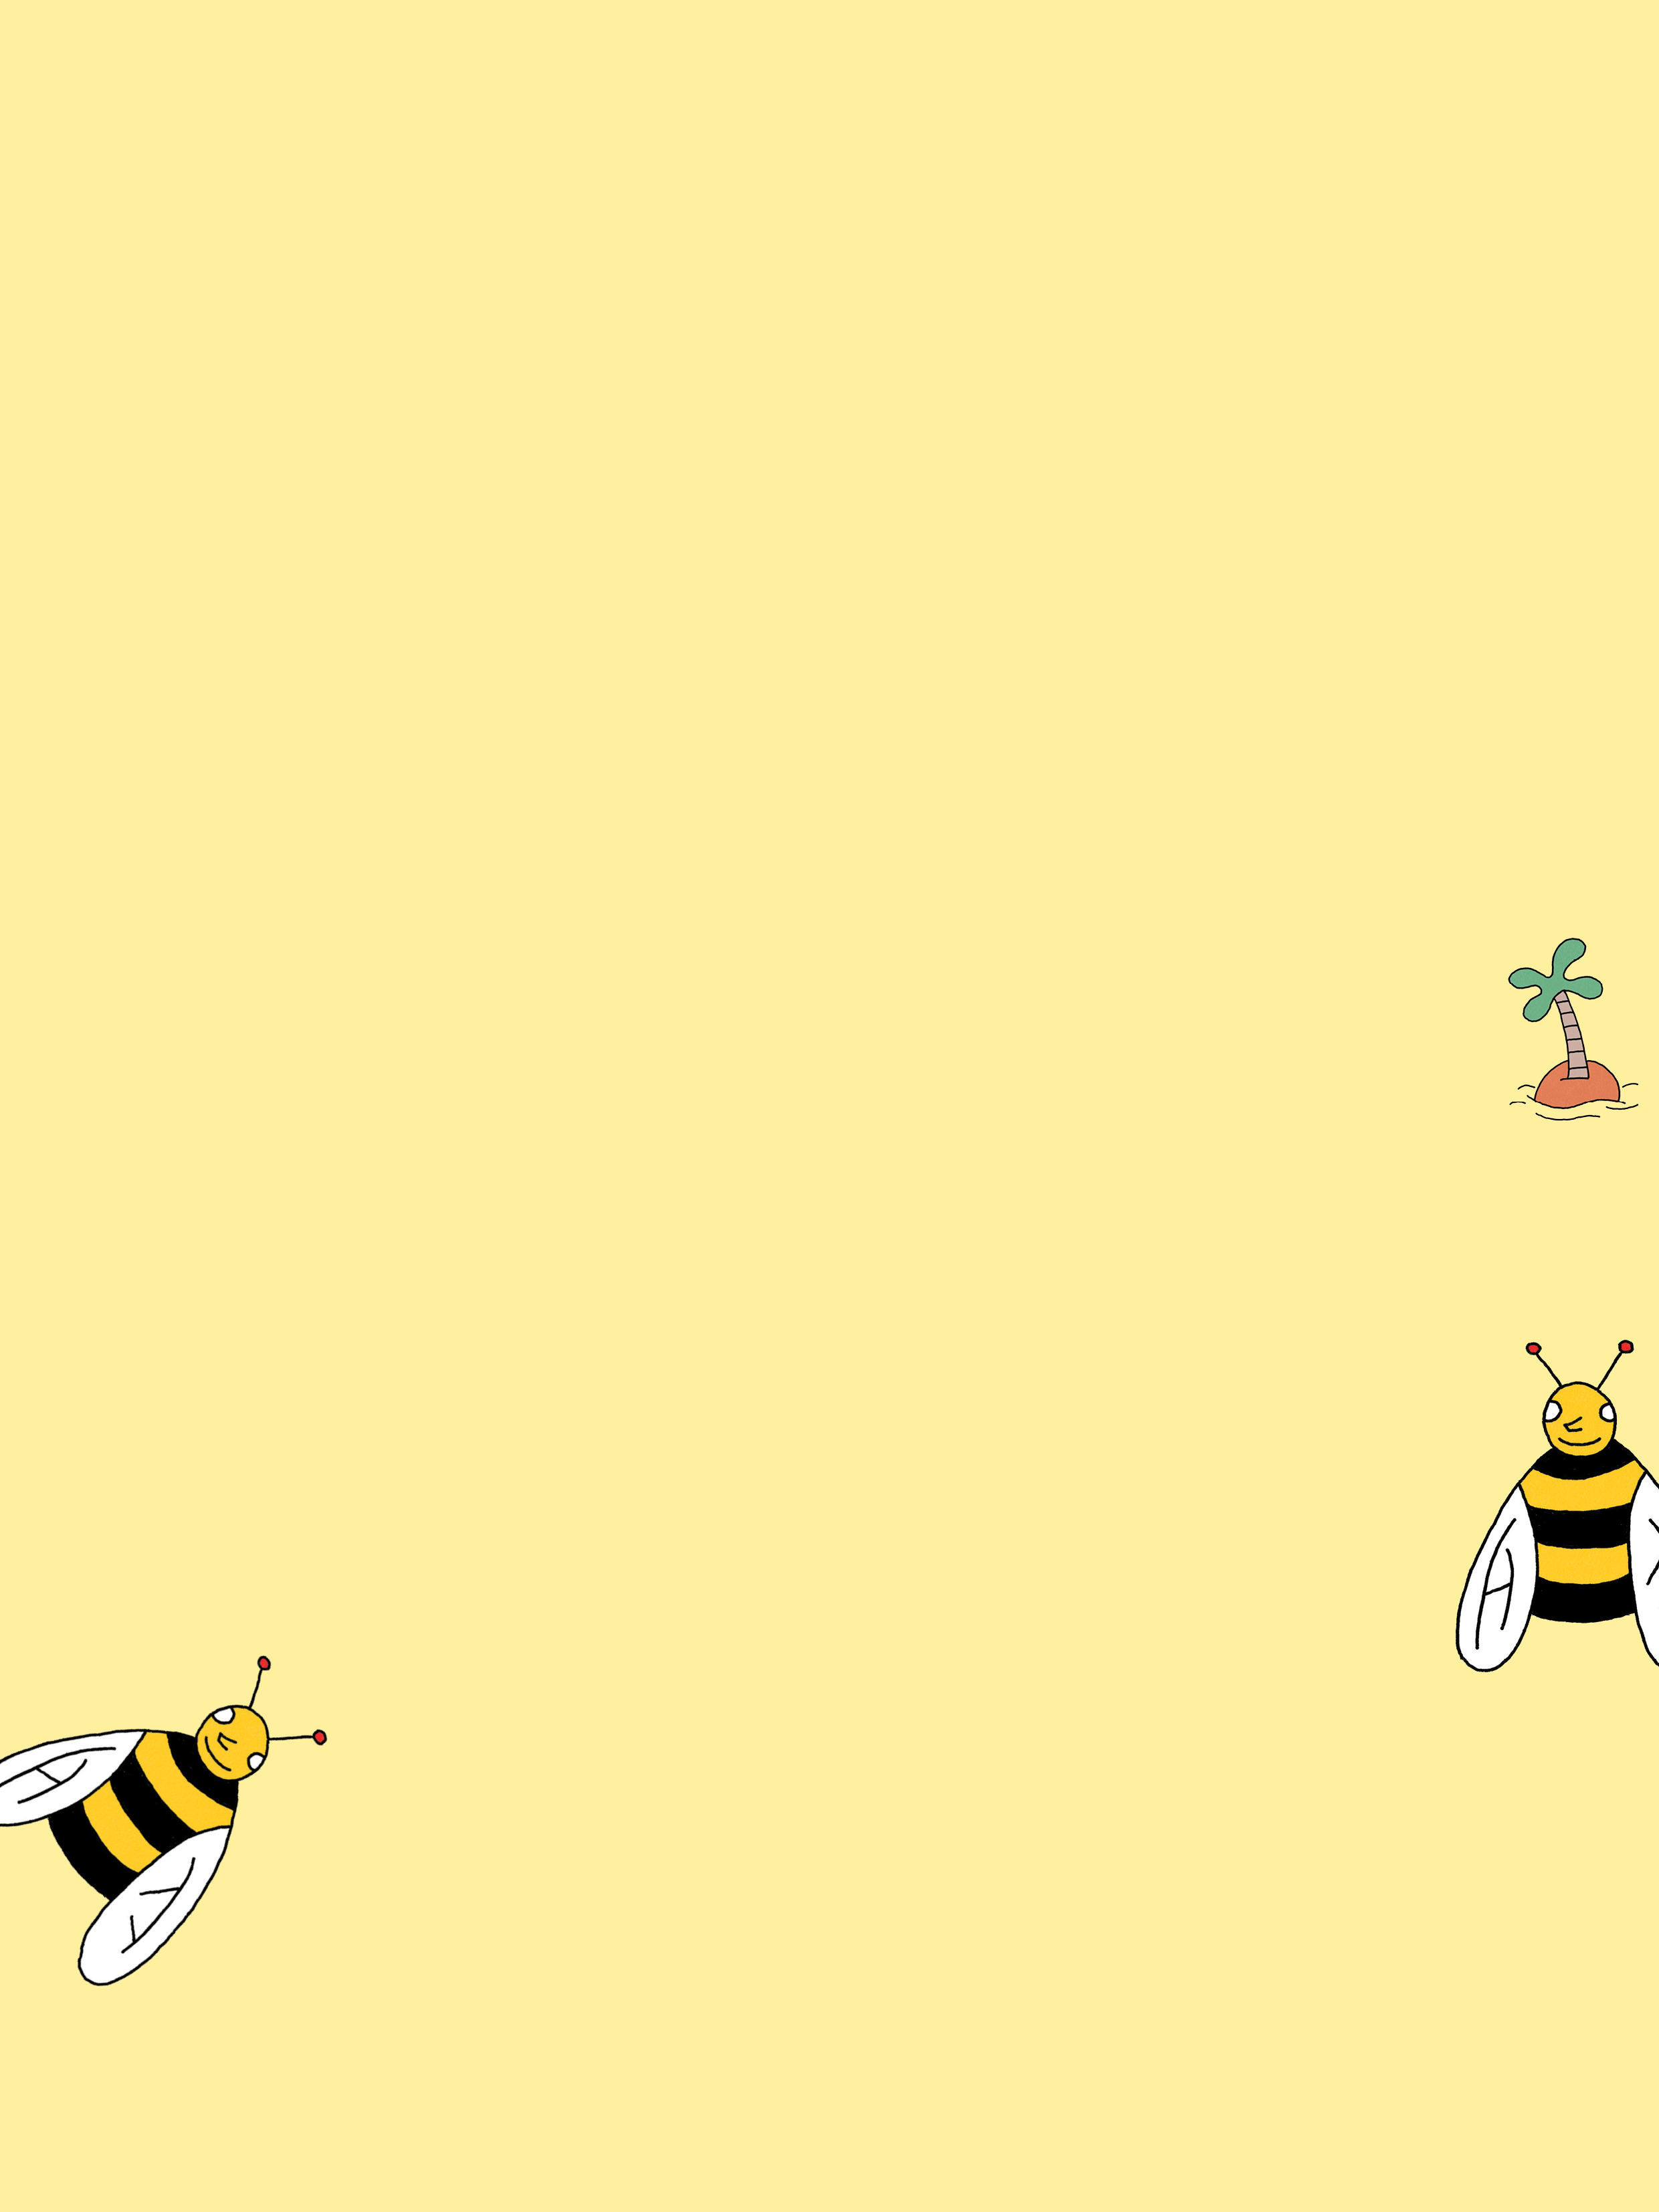
\includegraphics[scale=1]{watermarks/020.png}}

%\pagecolor{cyan!0!magenta!10!yellow!28!black!28!}

\newcommand{\AutorLivro}{Marcelo Cipis}
\newcommand{\TituloLivro}{Alfabeto de coisas}
\newcommand{\Tema}{Quotidiano de crianças nas escolas; nas famílias e nas comunidades (urbanas e rurais)}
\newcommand{\Genero}{Prescritivos: instruções; guias; manuais; ciclo de crescimento; ciclo de vida etc}
\newcommand{\imagemCapa}{./images/PNLD2022-020-01.png}
\newcommand{\issnppub}{978-65-86497-58-8}
\newcommand{\issnepub}{978-65-86497-72-4}
% \newcommand{\fichacatalografica}{PNLD0001-00.png}
\newcommand{\colaborador}{{Paulo Pompermaier e Renier Silva}}

\begin{document}

\title{\TituloLivro}
\author{\AutorLivro}
\def\authornotes{\colaborador}

\date{}
\maketitle

%\begin{abstract}\addcontentsline{toc}{section}{Carta ao professor}
%\pagebreak

\tableofcontents



\section{Sobre o livro}

%27 caracteres
\paragraph{O livro} 
``Alfabeto de coisas'' é um livro que apresenta o alfabeto da língua portuguesa. 

%822 caracteres
\paragraph{Descrição} 
A cada página há uma letra do alfabeto da língua portuguesa, à esquerda, e à direita,
palavra que começa com esta letra. Assim, temos ``abelha'', ``boi'' e ``casa'', por exemplo, 
para as três primeiras letras do alfabeto. 
Na direita, a primeira letra é grafada com a forma do elemento que a palavra designa. A vogal ``a'', então, terá
a forma de uma abelha, bem como o ``b'' terá a forma de um boi, o ``c'', de uma casa, e assim por diante. 
As ilustrações são lúdicas e a escolha do vocabulário está conforme a faixa etária
e o quotidiano das crianças. Terão, por exemplo, palavras adotadas pela língua
portuguesa que fazem parte do dia a dia, como ``yakissoba'', e partes do corpo humano, como ``olho''.

%411 caracteres
\paragraph{Competências} 
As crianças da \textbf{Creche \textsc{ii}} poderão trabalhar diversas competências
com este livro. Primeiro, a apresentação das letras que compõem o alfabeto
da língua portuguesa, tratados aqui de uma forma lúdica, permitirá 
uma familiarização mais fácil com o conteúdo. Vale a pena lembrar que o começo
da alfabetização é imprescindível a todas as outras etapas do letramento,
por isso é importante que o aprendizado se dê de forma eficaz, e para isso
a ludicidade deve permear todas as etapas do trabalho. No livro,
não são só os desenhos das coisas que imitam a forma das letras que
propõem isso, mas também as cores tornam o ambiente mais instigante e 
chamativo para os estudantes. Tudo para que o aprendizado seja o mais participativo
e prazeroso. 

%862 caracteres
\paragraph{Aprofundamento} 
Este material tem a intenção de contribuir para que você consiga desenvolver um trabalho aprofundado 
com esta obra na sala de aula. Você encontrará informações sobre o autor, sobre 
o gênero e sobre os temas trabalhados ao longo do livro. Apresentaremos também 
algumas propostas de trabalho para a sala de aula que você poderá explorar livremente, 
da forma que considerar mais apropriada para os seus estudantes. Para a prática 
da Literacia Familiar, oferecemos um guia que pode ajudar nas orientações aos 
responsáveis pela criança, para incentivar o gosto pela leitura e contribuir para 
que os estudantes desenvolvam em casa habilidades que serão importantes no momento 
da alfabetização. Por fim, você encontrará sugestões de livros, artigos e sites 
selecionados para enriquecer a sua experiência de leitura e, 
consequentemente, a de seus estudantes.


\section{Sobre o autor}

%532 caracteres
\paragraph{O autor} 
Marcelo Cipis nasceu em São Paulo, em 1959. 
Ingressou no mundo das artes plásticas em 1968, com participação em ateliês 
livres e aulas com artistas de diferentes modalidades. Atua sobretudo como 
ilustrador, desenhista e pintor deste 1977, tendo realizado trabalhos para 
livros, revistas e jornais.

\reversemarginpar
\marginparwidth=5cm

\marginnote{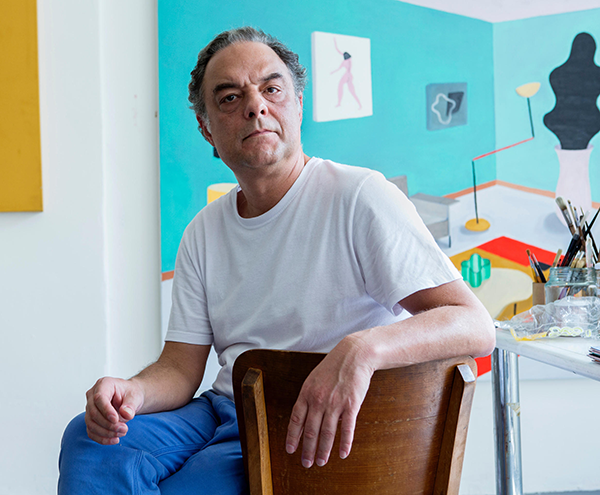
\includegraphics[width=\marginparwidth]{./images/PNLD2022-020-02.png}\\
O autor e ilustrador Marcelo Cipis (Arquivo pessoal)}

%313 caracteres
\paragraph{Publicações} 
Além de ter trabalhado na capa e ilustrações de diversos livros, 
publicou \emph{Era uma vez um livro}, pela Companhia das Letrinhas, \emph{530g de ilustrações}, pelo Ateliê Editorial e, com Antônio Malta, \emph{Viver é... e Namorar é...}, pela Martins Fontes.
%358 caracteres
\paragraph{Currículo} 
Formado em arquitetura pela fau-usp em 1982, participou dos Salões de Arte 
Contemporânea de São Paulo nos anos 1980 e da 21ª Bienal de São Paulo em 1991, 
além de outras mostras e workshops no Brasil e no exterior. Recebeu o Prêmio 
Jabuti de Ilustração em 1994 e uma bolsa da Pollock-Krasner Foundation em 2000, 
entre outros. Suas obras exploram diferentes combinações de formas geométricas 
e cores na representação lúdica de corpos e espaços.


\section{Sobre o gênero}

%55 caracteres
\paragraph{O gênero} O gênero deste livro é \textit{prescritivos}. 

\Image{No gênero prescritivo, o principal objetivo é instruir o leitor --- assim como a orientação de um dicionário. (Piqsels; Domínio público)}{PNLD2022-020-07.png}

%596 caracteres
\paragraph{Descrição} 
Textos do gênero prescritivo têm como característica principal instruir
o leitor. Extremamente comuns na vida quotidiana, eles estão presentes
sempre que se precisa de uma guia ou uma orientação. São estruturas 
que oferecem padrões: leis, que podem ser jurídicas, como um código
penal, ou gramaticais, como um dicionário ou uma gramática; a constituição
de um país etc. Seu conteúdo é, de alguma forma, imutável, ao menos até que seja
mudado. O significado de uma palavra no dicionário deve continuar o mesmo
até que um novo seja adicionado. Enquanto isso, o texto
estabelecido será aquele que tem valor absoluto.


%603 caracteres
\paragraph{Interação} 
Ainda que não sejam os gêneros privilegiados pela literatura
como as narrativas ou os poemas líricos, os textos prescritivos
têm uma grande importância para a vida em sociedade. A todo 
tempo estamos recorrendo a estas obras, em geral de consulta, para
sabermos como devemos agir, seja uma dúvida a respeito da ortografia ou 
dos significados de uma palavra, seja a respeito de um direito ou dever
enquanto cidadão. É de extrema importância, portanto, que as crianças
sejam o mais cedo apresentadas a este gênero, ainda que com a 
devida abordagem lúdica que a idade demanda. 

%862 caracteres
\paragraph{Competências} 
As competências trabalhadas numa obra do gênero prescritivo como o 
\emph{Alfabeto de coisas} são diversas. 
Primeiro, há uma apresentação à necessidade de se fazer as coisas de um 
determinado jeito. É o mundo das regras e convenções sociais: há um modo 
convencionadamente correto de se escrever as palavras. E a partir de letras 
se formam palavras, que representam coisas. Então temos outra competência, 
que é a descoberta de novos vocabulários. Mesmo que alguns desses objetos já 
fizessem parte do imaginário de algumas crianças, agoras eles passam
a ser associados a suas representações escritas, o que corrobora numa 
complexificação da realidade a partir deste novo universo. Ainda que 
pareça ser um gênero limitante, são os conhecimentos fixados nestas obras 
que permitem a expansão da criatividade com a garantia de que o outro irá 
entender já que as convenções são comuns.

\section{Temas}

\subsection{Quotidiano de crianças nas escolas; nas famílias e nas comunidades (urbanas e rurais)}

%136 caracteres
\paragraph{Abordagem} 
Apresentação do alfabeto da língua portuguesa por meio de uma linguagem lúdica. 
%206 caracteres
\paragraph{Descrição} 
A cada página é apresentada uma letra do alfabeto, acompanhada de uma palavra
que comece com a mesma letra e uma ilustração. São privilegiados
vocabulários que fazem parte do dia a dia das crianças na escola e nas
comunidades. 
%275 caracteres
\paragraph{Competências} 
Este tema relaciona-se, principalmente, ao campo de experiência 
``Escuta, fala, pensamento e imaginação'', descrito pela \textsc{bncc}, 
que tem como intuito aproximar as crianças das diferentes linguagens 
presentes no quotidiano por meio da escuta e da fala.

\section{Modelagem de aula}
A seguir você encontrará a descrição de uma aula modelo como exemplo 
prático de exploração do livro com estudantes. Esta seção apresentará 
orientações sobre como organizar a sala de aula para receber os 
estudantes, exercitar a interação verbal e prepará-los para o 
momento da leitura.

Em seguida, você encontrará a \textbf{Leitura dialogada}, um 
tópico destinado a te orientar para o momento específico da 
leitura com os estudantes. Por fim, no tópico 
\textbf{Propostas de atividades}, você encontrará ideias 
de práticas que pode explorar com as crianças em sala de 
aula após a leitura. 

Essas atividades podem ser trabalhadas de acordo com a 
disponibilidade do seu cronograma e fique à vontade para adaptá-las 
da forma que achar melhor para os seus estudantes. Cada turma é única 
e o seu conhecimento prático das características de cada aluno será 
essencial para definir a melhor forma de aplicar essas ideias. 

O objetivo deste manual é oferecer algumas ideias 
e inspirações para um trabalho que pode ser desenvolvido tanto 
a curto, quanto a médio e longo prazo. Sinta-se a vontade para 
personalizar a aula e torna-la sua, aplicando seus conhecimentos, sua 
personalidade e aproveite para fortalecer 
seu vínculo com a turma.


\subsection{Antes de ler}

\BNCC{EI02EO06} 
\BNCC{EI02EF03} 
\BNCC{EI02EF04} 
\BNCC{EI02EF06} 
\BNCC{EI02EF07} 
\BNCC{EI02EF08} 
\BNCC{EI02EF09}

%Alterar o nível escolar nesse parágrafo.
Como este trabalho será realizado com crianças da \textbf{Creche \textsc{ii}}, 
que ainda não têm muita intimidade com o livro enquanto objeto, você terá o 
papel de mediar este contato. 

Nosso objetivo é que os próprios estudantes possam manusear 
e explorar o livro de forma autônoma, mas, para que isto aconteça, você 
pode ajudar a tornar o caminho mais convidativo com atividades que tenham 
intencionalidade educativa. 

A \textsc{bncc} define intencionalidade educativa como ``organização 
e proposição, pelo educador, de experiências que permitam às crianças 
conhecer a si e ao outro e de conhecer e compreender as relações com a 
natureza, com a cultura e com a produção científica, que se traduzem nas 
práticas de cuidados pessoais (alimentar-se, vestir-se, higienizar-se), 
nas brincadeiras, nas experimentações com materiais 
variados, na aproximação com a literatura e no encontro com as 
pessoas''.\footnote{\textsc{bncc}, página 39}

É importante manter essa intencionalidade em mente não apenas na condução 
das atividades propostas neste manual, mas também para aproveitar as 
oportunidades espontâneas de construir conhecimentos que podem surgir durante 
a interação direta com os estudantes.

\begin{enumerate}
%836 caracteres
\item \textbf{O ambiente}\quad Antes de iniciar o trabalho com o livro, é importante que você 
prepare o ambiente para receber a turma. Como o trabalho com o livro terá 
três momentos (antes, durante e depois da leitura), seria interessante que você 
criasse um ambiente para cada etapa. Nas \textbf{Sugestões de referências complementares} 
você encontrará um artigo que discorre sobre a importância da organização da sala 
de aula para a educação infantil, que pode ser um bom guia para a criação desses 
ambientes. Para o momento antes da leitura, decore a sala de aula as letras
do alfabeto em emborrachado, preferencialmente, ou impressas em folhas.
É importante que tenhma cores chamativas e sejam bonitas. 

\Image{Pode ser utilizado um alfabeto emborrachado para o momento antes da leitura. (PxHere; Domínio público)}{PNLD2022-020-09.png}

%413 caracteres
\item \textbf{Primeira opção}\quad Utilize os primeiros 
momentos da aula para passear por essa área, chamando atenção para cada um 
das letras. Pergunte-lhes as pronúncias. É importante que todas as contribuições sejam ouvidas, então,
repita alto para todos sempre que alguém falar. Pergunte o que são essas coisas, 
para que servem cada uma. 

%632 caracteres
\item \textbf{Segunda opção}\quad Outra possibilidade para familiarizar 
as crianças com as letras que serão abordadas no livro é colocar uma música ambiente
de tom lúdico e divertido que fale do alfabeto. A ideia aqui não
é ainda apresentar diretamente o alfabeto às crianças,
mas deixá-las experimentar os estímulos sonoros com o corpo. 
Caso tenha um tapete de letras emborrachadas na sala, deixe-os à vontade 
sobre ele para pular, se jogar e o que mais quiserem, mas sempre
tomando cuidado para não se machucarem.
\end{enumerate}


\subsubsection{A interação verbal} 
Criar situações em que as crianças precisam dialogar diretamente com 
você é uma das práticas mais importantes de Literacia, pois elas estimulam 
o desenvolvimento linguístico, ampliam o vocabulário e reforçam a 
capacidade dos estudantes de compreenderem o que ouvem e se expressarem 
pela fala. O diálogo livre com a criança também reforça sua autoestima, pois 
a faz se sentir ouvida e valorizada pelo adulto, ao vê-lo prestar atenção 
no que ela tem a dizer. Portanto, sempre que possível, reserve um tempo na 
aula apenas para a interação verbal. 

Como esse tipo de interação é espontânea e intimamente atrelada ao 
desenvolvimento de cada estudante, nossas orientações não serão específicas. 
A ideia é que você adapte este momento de acordo com as respostas e os 
repertórios das crianças. É um momento de estreitamento de vínculos e, portanto, 
fique a vontade para ser espontânea e para explorar os tópicos que achar 
mais interessantes para a sua turma.

Inicie as conversas com naturalidade, seguindo os objetos de atenção das crianças. 
Você pode partir de objetos que estejam analisando
para iniciar um assunto e incentivar a se expressarem. Ainda
que a criança não fale corretamente, continue interagindo, pois a
intenção aqui é que ela perceba que outras pessoas estão respondendo à sua comunicação.

Fique atento a todas as formas de expressão: os gestos, as falas, as 
expressões faciais, para onde olham\ldots{} tudo pode ser explorado durante a conversa. 
Demonstre curiosidade sobre eles, seja um ouvinte entusiasmado e incentive que eles 
conversem entre si. Faça perguntas e construa a resposta junto com as crianças. 

A seguir, algumas dicas que podem contribuir para que a interação verbal 
seja produtiva em sua sala de aula: 

\begin{enumerate}
\item Sente-se no chão e brinque com eles, estabelecendo 
contato visual. Além das pequenas frases que conseguem formar,
vocalizações, gestos e expressões faciais podem ser boas formas
de comunicar.

\item Não se esqueça de que a conversa é uma troca e, portanto, evite
ficar falando sozinho ou desvalorizar as respostas das crianças
quando não conseguem formular frases completamente
articuladas. Nunca descarte uma tentativa de comunicação.

\item Evite utilizar falas negativas que desencorajam o diálogo. 
Se precisar que a turma 
corrija algum comportamento, explique claramente a razão e 
oriente com calma. Incentive positivamente as crianças e 
destaque o motivo de seus elogios. 

\item Aproveite alguns momentos durante a conversa para chamar 
a atenção das crianças para os sons das palavras e das letras que você 
acabou de usar ou que eles pronunciaram.  

\item Explore possibilidades de interação como apontar e 
nomear objetos, pessoas e animais ou fazer caretas, reproduzir sons de 
animais para que repitam, ensinar os nomes de partes do corpo, 
entre outras atitudes que estimulem a comunicação com a criança. 

\item Muitas dessas dicas poderão ser aproveitadas pela 
família durante a prática da Literacia Familiar. Portanto, 
se achar necessário, compartilhe algumas destas orientações 
com as famílias dos estudantes.
\end{enumerate}


\subsection{A leitura dialogada}
Este é o momento em que será realizada a leitura propriamente dita. 
Se possível, crie um \textit{cantinho da leitura} em sua sala de aula. Um 
ambiente confortável, de preferência em que todos se sentem no chão ou 
em pufes para que consigam enxergar as ilustrações do livro que está 
sendo lido e interagir com facilidade. Se houver possibilidade, mantenha 
sempre os livros da turma em uma altura da estante que permita fácil 
acesso para os estudantes ou guarde os livros em uma caixa que as crianças 
possam mexer com autonomia. É importante que elas tenham autonomia para 
acessar os livros e se sintam à vontade para pegá-los sempre que quiserem. 

\Image{É importante que o cantinho da leitura proporcione autonomia para as crianças. (Tânia Rêgo/Agência Brasil; CC BY-NC 2.0)}{PNLD2022-020-08.png}

Outra possibilidade de ambiente para esta leitura, se a escola permitir, 
é efetuar essa leitura ao ar livre, embaixo de uma árvore, onde as crianças 
possam ouvir os sons dos pássaros e sentir o cheiro da grama. Sair da sala 
de aula pode oferecer um ótimo leque de experiências aos seus estudantes e 
reforçar a conexão entre a natureza do livro e a realidade.  

Reserve uma boa parte da aula para o momento da leitura com os estudantes, 
pois é importante que esse momento aconteça sem pressa. O objetivo da 
leitura dialogada é que seja uma leitura em bate-papo. A criança deve 
assumir um papel ativo na leitura, mesmo que ainda não seja capaz de 
ler sozinha. Além de promover o gosto pela leitura, esta prática estimula 
o desenvolvimento da linguagem, enriquece o vocabulário e 
aumenta o conhecimento de mundo.

%Especificar o livro.
No caso de ``Alfabeto de coisas'' o diálogo durante a leitura
é importante pois as crianças ainda não foram alfabetizadas 
e não têm ainda familiaridade com as letras. Por isso, 
você deve interagir com eles durante toda a 
leitura, fazendo perguntas e partindo de detalhes do livro para 
levantar novas questões. 

A seguir, algumas orientações para aproveitar este momento: 

\begin{enumerate}
%177 caracteres
\item \textbf{Como começar}\quad Sente-se em um lugar acessível, 
onde todos conseguirão ouvir bem a sua leitura e enxergar as ilustrações 
quando você estiver mostrando o livro ou eles estiverem manuseando-o. 
Antes de abri-lo, chame a atenção dos estudantes para a capa. 
Faça perguntas como: 

\begin{itemize}
\item Sobre o que vocês acham que é esse livro?
\item Quais cores tem aqui na capa?
\item Que letras são essas?
\end{itemize}

Estas perguntas te ajudarão a avaliar repertório das crianças. 
Não há problema se as perguntas que você fizer não forem respondidas pelos 
estudantes. Você mesma pode respondê-las de forma simples e articulada. Se achar 
conveniente, peça que repitam algumas palavras com você e valorize tentativas 
de imitar a sua fala. 
 
%230 caracteres
\item \textbf{Manuseio}\quad Deixe que as crianças manuseiem o livro 
e explore com elas todos os elementos que o compõe. Mostre o que é a 
capa e onde estão as páginas. Leia o título do livro em voz alta, seguindo 
a leitura com o dedo, indicando as letras. 

%495 caracteres
\item \textbf{Diálogo}\quad A cada página ou a cada nova letra,
chame a atenção dos alunos. Faça perguntas como:

\begin{itemize}
\item O que é isso?
\item A abelha faz que barulho?
\item E o gato?
\item Que palavra parece com olho?
\end{itemize}

Você pode mostrar imagens ou vídeos dos animais ou objetos
apresentados no livro. Incentive os alunos a entrar
em contato com o que está sendo apresentado por meio da 
elaboração de frases. 

%346 caracteres
\item \textbf{Escuta}\quad Elogie atitudes positivas, como 
tentar tomar o papel central na leitura ou dar exemplo de outras
palavras que eles conhecem. Não force a leitura. Se as crianças 
estiverem cansadas, faça outra atividade e retorne depois. 

%935 caracteres
\item \textbf{Leitura}\quad Faça perguntas e comentários que aumentem o 
interesse e aticem a curiosidade e imaginação das crianças. 

\begin{itemize}
\item A é de abelha e de mais o quê? A de Ana também!
\item B de boi e de mais o quê? B de Bruna!
\item C de casa e de comida! Do que mais?
\end{itemize}

Não tenha pressa em passar as páginas. Como os alunos ainda não foram 
alfabetizados, eles podem levar algum tempo para associar a letra
ao som. Faça as perguntas listadas acima e espere que eles 
pensem. Se não houver nenhuma resposta dentro do esperado,
dê você um exemplo, priorizando palavras do quotidiano das crianças.

Também não deixe que eles fiquem sem entender do que se trata cada frase. Crie 
um ambiente amigável onde a criança se sinta à vontade para fazer 
perguntas e comentários durante a leitura.

\includepdf[nup=2x3, 				% grid
			%offset=-15mm -5mm, 	% posição
			scale=.8, 				% tamanho da página
            delta=4mm 4mm, 			
            frame,
            pages={4-5,16-17,40-41}]{./pdfs/\jobname_MIOLO.pdf}




%382 caracteres
\item \textbf{Interação}\quad Nomeie os elementos das ilustrações 
do livro, apontando para elas com o dedo. Destaque os sons de algumas 
palavras. Interrompa a leitura em alguns momentos e peça que 
os estudantes repitam palavras, como \textit{yakissoba}, \textit{jacaré}, \textit{árvore}. Se possível, 
leia a mesma palavra várias vezes.
\end{enumerate}


\subsection{Propostas de atividades}

\BNCC{EI02EO04} 
\BNCC{EI02CG05} 
\BNCC{EI02EF03} 
\BNCC{EI02ET02} 
\BNCC{EI02ET01} 
\BNCC{EI02ET05} 

\begin{enumerate}
%700 caracteres
\item \textbf{Como começar}\quad Após a leitura dialogada, é hora de criar 
atividades que proporcionem aos estudantes experiências novas a partir da história 
que acabaram de conhecer. Nesta idade é fundamental explorar os sentidos da criança e 
ajudá-lo a experimentar a história que acabou de conhecer de formas diversas. Se achar 
conveniente, convide os estudantes a se sentarem em roda. 

%650 caracteres
\item \textbf{O ambiente}\quad  
Para esta atividade, você pode reaproveitar a ambientação da 
atividade de pré-leitura, com os emborrachados das letras
do alfabeto e as letras coloridas impressas. Tanto a sala
de aula quando um ambiente externo como a área de diversão
podem ser usados. 

%950 caracteres
\item \textbf{A atividade}\quad “Alfabeto de coisas” é um livro
que trabalha sobretudo com as faculdades da linguagem escrita que
está neste momento sendo apresentada às crianças. Uma forma de 
ligar a língua escrita à oral é por meio de um telefone sem fio.
Ao fim da brincadeira, quando a palavra for passada por todos,
você deve mostrá-la escrita. Assim, eles perceberão 
a função estabilizante da escrita de modo prático.

Diga aos estudantes que eles irão experimentar uma nova brincadeira.
Pergunte quem já brincou de telefone sem fio. Peça que alguém que já
conheça a brincadeira tente explicá-la aos demais colegas.
Após a tentativa, explique você como funcionará: você vai falar
no ouvido de um aluno uma das palavras estudadas no livro
e ele deve passar para a pessoa à sua esquerda ou direita, 
que irá continua no mesmo sentido. Assim continuamente até que chegue à última
pessoa, que deve falar a palavra em voz alta. 

\Image{A brincadeira de telefone sem fio pode ser interessante para ligar a língua escrita à oral. (Mack Male; CC-BY-SA-2.0)}{PNLD2022-020-10.png}

%550 caracteres
\item \textbf{Interação}\quad O livro pode e deve ser 
manipulado pelos estudantes. Incentive que eles tentem ler
todas as palavras na ordem que estão apresentadas. 
Elogie as tentativas de reprodução sem deixar de 
corrigir as pronúncias. Não esqueça que sua postura deve
ser sempre estimulante. 
\end{enumerate}


\section{Literacia familiar}
O \textsc{pna} dá destaque especial para a importância do envolvimento da família 
no processo pedagógico nesta faixa etária e denomina Literacia Familiar o conjunto 
de experiências e práticas relacionadas à linguagem (oral, escrita ou lida) vivenciadas 
com os cuidadores. 

Essas estratégias podem começar a ser colocadas em prática desde a 
gestação e continuar até o final da adolescência. São práticas simples e divertidas 
que estimulam o desenvolvimento de quatro atividades fundamentais: ouvir, falar, 
ler e escrever que criam momentos de afeto e interação para a família. 

Para que esse trabalho conjunto entre escola e família funcione, é 
fundamental que a escola esteja em constante diálogo com os responsáveis e 
você consiga orientá-los. Um grupo em aplicativos de mensagens instantâneas ou um 
grupo de e-mails são saídas viáveis para que a comunicação se estabeleça e pode ser 
uma forma útil das famílias compartilharem suas vivências e trocarem sugestões 
de abordagens, sempre contando com a sua mediação. 

Com o objetivo de incentivar 
a prática da \textit{literacia familiar}, se possível, organize um rodízio entre os familiares 
das crianças para emprestar o livro da biblioteca da turma. Neste caso, crie um caderno 
de registro e estabeleça períodos para cada família ficar com o livro. É importante 
que os familiares compreendam a seriedade deste compromisso, pois o livro pertence 
ao acervo da sala e, portanto, deve ser bem cuidado e devolvido na data acordada. 

Se não for possível garantir o acesso direto dos cuidadores da criança ao livro, 
grave um vídeo direcionado a eles, contando a história e apresentando algumas 
das ilustrações. O importante é que os familiares saibam com clareza qual livro 
está sendo trabalhado, a história contada e se sinta seguro para explorar as temáticas 
do livro com a criança. Orientações claras e a manutenção do canal de comunicação com 
os responsáveis é essencial para que eles se sintam seguros e à vontade para fazer perguntas 
se tiverem dúvidas. 

Neste manual, você encontrará algumas práticas que podem ser 
recomendadas aos familiares para ajudá-los a expandir e aprofundar o trabalho 
que você iniciou em sala de aula.


\subsection{Importância da leitura}
Na escola, aprendemos a ler letras, mas é importante ter em mente que nós 
lemos o mundo desde muito pequenos: “lemos” os animais que passam pelos nossos 
quintais, a expressão no rosto dos nossos familiares, as cores que pintam o céu 
em um fim de tarde. 

Vamos aprendendo, ao longo da vida, a interpretar acontecimentos 
e sons que escutamos e a utilizá-los para nossa comunicação. Aprender a ler textos e 
escrevê-los expande a nossa leitura do mundo, pois permite que sejamos capazes de 
interpretar um código e experimentar, a partir dele, novas experiências e conhecimentos. 

O simples contato com os livros já permite um leque grande de sensações: 
sentimos as texturas, as formas, vemos as cores do livro, escutamos o som da página 
virando e o som da voz do narrador, se a história estiver sendo lida em voz alta. Para uma criança, são experiências que podem contribuir diretamente com o desenvolvimento psicomotor 
e cognitivo. 

Nosso papel, enquanto mediadores de leitura, é contribuir para que essas 
sensações sejam associadas a momentos positivos, de construção de 
conhecimento e exercício de imaginação. 

Com os livros, podemos conhecer mais da história humana, descobrir informações 
novas sobre sociedades diferentes da nossa, imaginar situações e contextos inéditos 
para nós e aumentar o nosso repertório. São por meio deles que melhoramos nossa 
capacidade de interpretação, de expressão, de análise e senso crítico. Boas habilidades 
leitoras podem contribuir para o desenvolvimento de um estudante em todas as outras 
disciplinas, pois exercem influência direta na forma como absorvemos e 
construímos conhecimento.


\subsection{O papel da família na formação do leitor}
A família é peça fundamental na formação do leitor, pois é ela quem primeiro 
ensina a criança a ler. Não apenas os textos escritos, mas a ler o mundo, a 
interpretar os estímulos que a cercam, a construir seu próprio vocabulário e a 
comunicar seus pensamentos e necessidades.

O universo das letras é muito presente na vida das crianças antes mesmo de sua 
entrada na escola. Aparece nas histórias e ilustrações do livro que o cuidador 
lê ao colocá-la para dormir, nas situações em que vê os responsáveis se comunicarem 
pela escrita ou nos textos que podem permear seu cotidiano (nos outdoors, na 
televisão, no celular, manuais de instrução entre outros). 

Os familiares têm, 
portanto, uma ótima oportunidade de apresentar a leitura com leveza, de forma 
prazerosa, associado ao contexto em que a criança vive e à momentos de diversão. 
Você poderá orientar os pais nesta tarefa, ensinando-os com este guia a aproveitar 
as oportunidades para trabalhar a Literacia com a criança.


\subsubsection{Práticas de literacia familiar} 

São muitas as experiências que a prática da \textit{literacia familiar} 
pode oferecer às crianças. A seguir, explicamos cada uma delas para que você possa, 
se achar necessário, compartilhar com os responsáveis enquanto estiver orientando-os: 

\paragraph{Interação verbal} Aumentar a quantidade de conversas com as 
crianças, fazendo perguntas para incentivar o diálogo.

\paragraph{Leitura dialogada} Interagir com a criança durante a leitura 
em voz alta, criar expectativa sobre o livro, chamar a atenção para detalhes 
das ilustrações e comentar o enredo.

\paragraph{Narração de histórias} Interagir com a criança enquanto 
estiver narrando uma história, por exemplo, incluindo-a na ação, utilizando 
marionetes ou permitindo que ela complete a narrativa.

\paragraph{Contatos com a escrita} Apresentar as letras para as 
crianças, incentivar que tentem escrever ou ler, ajudá-los a desenhar letras, 
entre outras formas de incentivar o contato com as palavras.

\paragraph{Atividades diversas} Qualquer atividade com a criança 
pode ser utilizada para contribuir para a alfabetização. Jogos, brincadeiras, 
instrumentos musicais, canto, dança, passeios e viagens oferecem boas 
oportunidades de aprendizado.

\paragraph{Motivação} Atitudes que motivem as crianças à envolver-se com 
o mundo da leitura e da escrita.

\subsection{Exercitando a literacia familiar}

\BNCC{EI02ET03} 
\BNCC{EI02EF07} 
\BNCC{EI02EF08} 
\BNCC{EI02EF03} 
\BNCC{EI02EF05} 

\begin{enumerate}
%700 caracteres
\item \textbf{Como começar}\quad Como se trata de um livro
prescritivo e não narrativo, talvez os pais e cuidadores
se sintam um pouco perdidos em relação a como usar o material
com as crianças. Neste caso, deixe-lhes à vontade para 
utilizar o material de formas diversas; desde uma simples leitura
das palavras em ordem alfabética, até experimentos mais criativos,
como indicaremos mais abaixo. Se achar conveniente, compartilhe com 
os familiares algumas dicas das seções Interação verbal 
e Leitura dialogada e as indicações nas Referências Complementares 
para ajudá-los a explorar as possibilidades oferecidas pelo livro. 

%650 caracteres
\item \textbf{Leitura}\quad A família pode continuar 
explorando os temas apresentados pelo livro. Os familiares podem explorar 
elementos do cotidiano que se relacionam à história e indicar a conexão 
entre o que viram na ilustração e a realidade. Durante a leitura 
de cada letra, elementos do ambiente podem ser indicados. Por exemplo,
se a leitura estiver sendo feita na cozinha, o familiar pode indicar,
na letra ``a'' objetos como ``arroz'', ``armário'', ``abóbora''; no
quintal, ``árvore'', ``azul'' (falando da cor do céu) \dots{} As possibilidades
são diversas dentro dos próprios cômodos da casa e ainda mais
caso haja a possibilidade de ir a um espaço público, como um parque,
uma praia, um zoológico\dots{}

%1073 caracteres
\item \textbf{Instrução}\quad Para trabalhar junto ao livro,
os familiares podem apresentar uma das músicas do alfabeto
indicadas nas Sugestões de referências complementares.
Cantem juntos até que a criança aprenda a ordem das letras.
Quando ela tiver dominado todo o alfabeto, peça que ela leia
o livro para outro familiar, amigo ou vizinho. Mesmo que ela
apresente algumas dificuldades na pronúncia das palavras, é importante 
que os mais velhos ouçam com atenção e valorizem todas as tentativas 
da criança. Afinal, ao tentar ler por si só, ela manipulará o livro, 
treinará a coordenação motora, conhecerá as texturas do objeto e
poderá imitar a forma como o adulto lê, treinando a fala. 
\end{enumerate}

 
\section{Sugestões de referências complementares}

\subsection{Livros} 

\begin{itemize}
\item \textsc{lins}, Guto. Livro infantil? projeto gráfico, metodologia, subjetividade. São Paulo: Rosari, 2002.
Livro que aborda a importância das escolhas visuais (ilustração, projeto gráfico, lettering) na literatura infantil.  

\item \textsc{hunt}, Peter. Crítica, teoria e literatura infantil. São Paulo: Cosac Naify, 2010.
Livro sobre crítica de literatura infantil que contêm definições de livro ilustrado e livro imagem. 
\end{itemize}

\subsection{Artigos}

\begin{itemize}

	\item \textsc{carvalho}, Lydiane Fonseca de. \emph{Poesia na sala de aula: as contribuições da poesia na formação
	do leitor literário.} Disponível em: \url{http://www.cchla.ufrn.br/shXIX/anais/GT12/POESIA_ARTIGO_HUMANIDADES.pdf}. Acesso em 23 ago. 2021.
	Artigo acadêmico que discorre sobre as contribuições da poesia na formação de crianças.
	\item \textsc{sardelich}, Maria Emilia. \emph{Leitura de Imagens, Cultura Visual e Prática Educativa.} 
In: Cadernos de Pesquisa. V.36, n.128, p.451-472, mai/ago.2006. Disponível em: \url{https://www.scielo.br/pdf/cp/v36n128/v36n128a09}. 
Acesso em 29 abr 2021. 
Artigo acadêmico que discorre sobre a importância de trabalhar cultura 
visual na educação na sociedade contemporânea. 

\item \textsc{pranke}, Marha Elfrida. \emph{Organização dos espaços da sala de aula na Educação Infantil.} Disponível em: 
\url{http://centraldeinteligenciaacademica.blogspot.com/2016/04/organizacao-dos-espacos-da-sala-de-aula.html}. Acesso em 04 mai 2021. 
Artigo acadêmico que discorre sobre a importância da rotina e de criar ambientes dentro da sala de aula na Educação Infantil.  
\end{itemize}

\subsection{\textit{Sites}}

\begin{itemize}
\item Vídeos “Conta pra mim” no site do \textsc{pna}. Disponível em: \url{http://alfabetizacao.mec.gov.br/contapramim}. 
Acesso em 13 abr. de 2021.
Página do \textsc{mec} com vídeos sobre leitura dialogada que visam incentivar a Literacia Familiar. Muitas das 
técnicas, explicações e materiais disponíveis nessa página podem ser utilizados em aula, mas o site também 
pode ser uma ótima indicação para ajudar a direcionar os cuidadores dos estudantes a praticar 
a literacia familiar e leitura dialogada.

\item Vídeo “Livros de imagem: como utilizar com as crianças?” do canal Conta Outra. Disponível em Youtube. 
Acesso em 14 abr. 2021. 
Neste vídeo, a pedagoga Bel explica o que são livros de imagem e faz sugestões para mediar a leitura com 
crianças. Se você achar conveniente, esse vídeo pode ser recomendado aos familiares da criança 
para inspirá-los na leitura dialogada. 

\end{itemize}

\subsection{Para os estudantes}

\begin{itemize}
\item Música ``\textsc{abc}'' do canal Galinha Pintadinha. Disponível no Youtube. \url{https://www.youtube.com/watch?v=JNA4-mjSf00}. Acesso em 28 ago. 2021.


\end{itemize}


\section{Bibliografia comentada}

\subsection{Livros}

\begin{itemize}
\item \textsc{brasil}. Ministério da Educação. Base Nacional Comum Curricular. Brasília, 2018.
Consultar a \textsc{bncc} é essencial para criar atividades para a turma. Além de especificar 
quais habilidades precisam ser desenvolvidas em cada ano, é fonte de informações sobre 
o processo de aprendizagem infantil. 

\item \textsc{brasil}. Ministério da Educação. Secretaria de Alfabetização. Conta pra mim: Guia de Literacia Familiar. 
Brasília: \textsc{mec, sealf}, 2019. Disponível em: \url{http://alfabetizacao.mec.gov.br/images/conta-pra-mim/conta-pra-mim-literacia.pdf}
Este guia é voltado aos pais e oferece explicações em uma linguagem bastante acessível e detalhada as práticas de Literacia Familiar, 
como praticar leitura dialogada, como narrar histórias, como exercitar interação oral, formas de proporcionar contatos com a escrita à criança etc. 
 
\item \textsc{brasil}. Ministério da Educação. Secretaria de Alfabetização. \textsc{pna} Política Nacional de Alfabetização/Secretaria 
de Alfabetização. Brasília: \textsc{mec, sealf}, 2019.
Um guia fundamental para trabalhar pré-alfabetização e alfabetização de estudantes, que ressalta a importância da Literacia e da Numeracia. 


\end{itemize}


\subsection{Artigos}

\begin{itemize}
\item \textsc{costa}, A. C. C.; \textsc{santos netos}, J. A.; \textsc{bortolin}, S; \textsc{pereira}, Ana Paula. O livro de imagem e a mediação na escola. 
In \textsc{vii secin}, Universidade de Londrina. Disponível em \url{http://www.uel.br/eventos/cinf/index.php/secin2017/secin2107/paper/viewFile/445/296}. 
Acesso em 29 abr 2021. 
Esse artigo reflete sobre a importância de se apresentar livros de imagem para os estudantes na escola para que as crianças aprendam a ler imagens. 

\item \textsc{nannini}, P. B. R.; \textsc{medeiros}, J. P. S.; \textsc{ribeiro}, J. M. Leitura em cena: Vivências em sala de aula com livro de imagens. 
Literartes, n. 3, p. 82-101, 2014. DOI: 10.11606/issn.2316-9826.literartes.2014.89204. 
Disponível em \url{https://www.revistas.usp.br/literartes/article/view/89204/92115}. Acesso em 29 abr. 2021. 
Artigo acadêmico sobre um trabalho utilizando o mesmo livro de imagem com crianças da educação infantil e ensino médio. 
É uma forma interessante de perceber que a leitura de imagens pode ser explorada com qualquer faixa etária. 
\end{itemize}

% 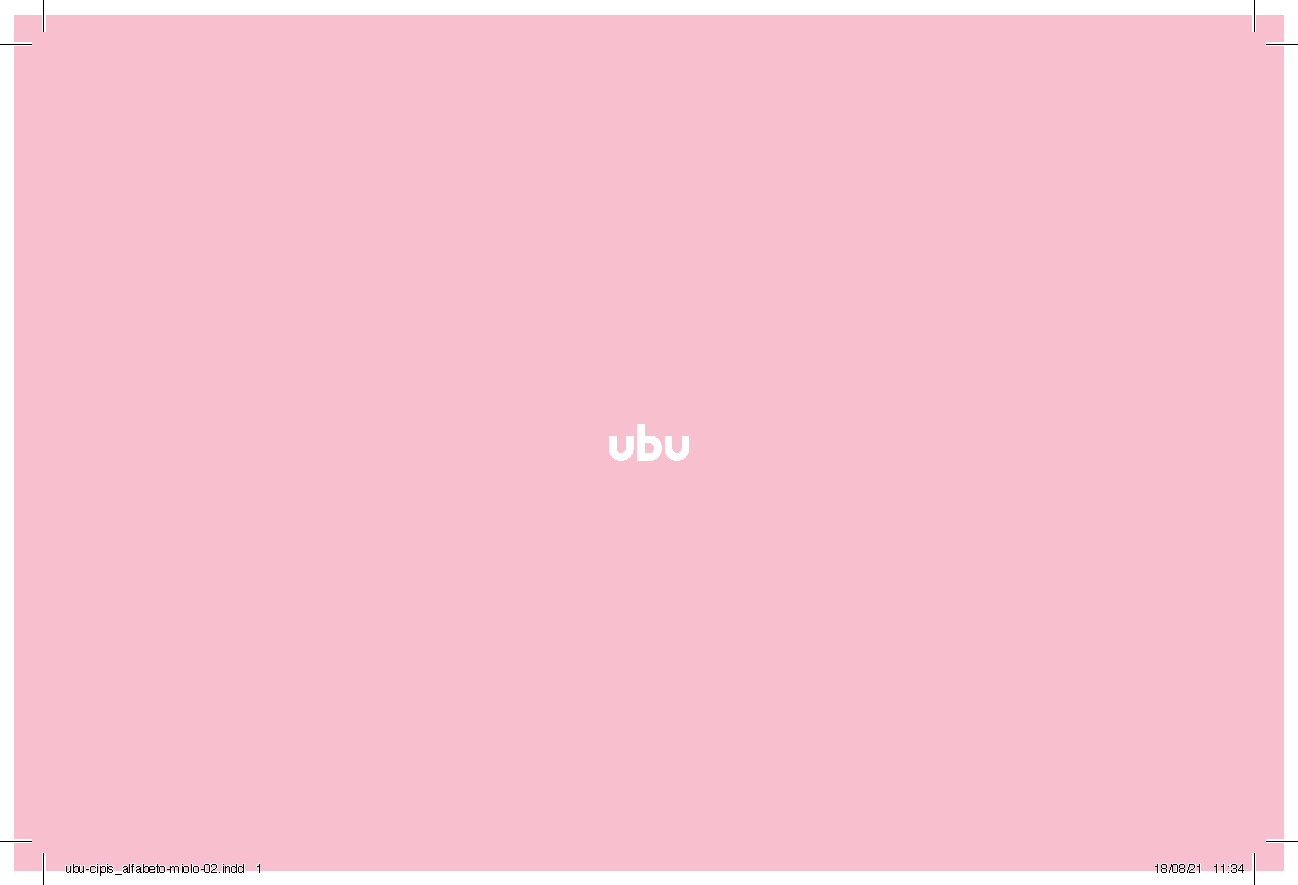
\includepdf[nup=2x2, 					% grid
			% offset=-15mm -5mm, 		% posição
			% scale=.8, 				% tamanho da página
            % delta=4mm 4mm, 			
            % frame,
            % pages={1-4}]{pdfs/PNLD2022-020_MIOLO.pdf}

\end{document}
